% LaTeXin \input-komentoja voi antaa sisäkkäin. Tyypillisesti jokaisella kappaleella on oma tiedostonsa, joka sisällytetään \input-komennolla päätiedostosta. Luvut voivat jakautua useampaan alitiedostoon pituudesta yms. riippuen. 
\part{Eulerin elämä ja teot}
% Kandin- tai pro gradu -tutkielmissa ei yleensä käytetä \part-komentoa. Tässä tapauksessa sitä käytetään, jotta \chapter-komentoa voidaan käyttää kuten normaalissa gradussa.
\chapter{Johdato}
\label{cha:euler}

Leonhard Euler (1707--1783) oli sveitsiläinen matemaatikko ja fyysikko, joka on saanut nimensä niin matematiikan kuin tietojenkäsittelytieteenkin historiaan. Tässä luvussa esitellään muutama Eulerin kuuluisa saavutus.

\chapter{Eulerin identiteetti}
\label{cha:eulerin-identiteetti}

\emph{Eulerin identiteetti} on seuraava yhtälö:
\begin{equation}
  \label{eq:euler_id}
  \e^{i\pi}+1=0\; .
\end{equation}
Identiteettiä \eqref{eq:euler_id} kutsutaan usein \enquote{matematiikan kauneimmaksi kaavaksi} \citep{reid06zero}. Se sisältää viisi tärkeää lukua: $0$:n, $1$:n, $\e$:n, $i$:n ja $\pi$:n. Näistä kolme viimeisintä on määritelty taulukossa~\ref{tab:vakiot}. 

\begin{table}
  \centering
    \caption{Tärkeitä matematiikan vakioita}
  \label{tab:vakiot}
  \begin{tabular}{@{}Lp{0.5\textwidth}R@{}}
    \toprule
    \text{symboli} & merkitys & \text{arvo}\\
    \midrule
    \e & Neperin luku, $\lim_{n\to\infty}(1+1/n)^n$ & \approx 0{,}577 \\
    \pi & ympyrän kehän ja halkaisijan suhde & \approx 3{,}142 \\
    i & imaginaariyksikkö & \sqrt{-1} \\
    \bottomrule
  \end{tabular}
\end{table}

Eulerin identiteetti seuraa Eulerin yhtälöstä.

\begin{theorem}[Eulerin yhtälö]
  \label{thm:euler_thm}
  Kaikille $x\in\R$ pätee, että
  \begin{equation}
    \label{eq:euler_thm}
    \e^{ix}= \cos x + i \sin x\; .
  \end{equation}
\end{theorem}

\begin{proof}
  Eulerin yhtälön todistus perustuu Taylorin sarjoihin. Eksponenttifunktion $\e^x$, sinifunktion $\sin x$ ja kosinifunktion $\cos x$ sarjaesitykset ovat
  \begin{align}
    \e^x &= 1 + x + \frac{x^2}{2!} + \frac{x^3}{3!} + \cdots \label{eq:exp_taylor}  \\
    \sin x &= x - \frac{x^3}{3!} + \frac{x^5}{5!} - \frac{x^7}{7!} + \cdots \label{eq:sin_taylor} \\
    \cos x &= 1 - \frac{x^2}{2!} + \frac{x^4}{4!} - \frac{x^6}{6!} + \cdots \label{eq:cos_taylor} \; ,
  \end{align}
  missä $x\in \R$. Kompleksiluvulle $z\in\mathbb{C}$ vastaavat sarjat saadaan korvaamalla $x$ muuttujalla $iz$. Näin sijoittamalla saadaan
  \[
    \begin{split}
      \e^{iz} &= 1 + iz + \frac{(iz)^2}{2!} + \frac{(iz)^3}{3!} + \frac{(iz)^4}{4!} + \cdots \\
      & =1 + iz - \frac{z^2}{2!} - \frac{iz^3}{3!} + \frac{z^4}{4!} + \frac{iz^5}{5!} - \frac{z^6}{6!} - \frac{iz^7}{7!} + \frac{z^8}{8!} + \cdots \\
      &= \left(1 - \frac{z^2}{2!} + \frac{z^4}{4!} - \frac{z^6}{6!} + \frac{z^8}{8!} + \cdots\right)
      + i\left(z - \frac{z^3}{3!} + \frac{z^5}{5!} - \frac{z^7}{7!} + \cdots \right) \\
      &= \cos z + i\sin z\; ,
    \end{split}
  \]
  missä ensimmäinen yhtälö saadaan suoraan \eqref{eq:exp_taylor}:sta, toinen saadaan kirjoittamalla $(iz)^n = i^nz^n$ ja muistamalla, että $i^2 = 1$, kolmas yhtälö saadaan ryhmittelemällä termit uudellen ja neljäs seuraa yhtälöistä \eqref{eq:sin_taylor} ja \eqref{eq:cos_taylor}.
\end{proof}

\begin{proof}[Eulerin identiteetin todistus]
  Sijoitetaan $x=\pi$ Eulerin yhtälöön ja saadaan $\e^{i\pi} = \cos\pi + i\sin\pi$. Trigonometriasta muistamme, että
  \begin{align}
    \cos\pi &= -1 \\
    \intertext{ja}
    \sin\pi &= 0\; ,
  \end{align}
  joten $\e^{i\pi} = -1$, mistä saadaan identiteetti
  \[
    \e^{i\pi}+1 = 0\; .
  \]
\end{proof}


\chapter{Eulerin kehä ja Königsbergin siltaongelma}
\label{cha:eulerin_keha}

% Makro \kaliningrad on määritelty aiemmin.
% Oikea määrittely riippuu käytettävästä LaTeXin versiosta.
Königsbergin (nyk. \kaliningrad (Kaliningrad)) kaupungin läpi virtaa joki, jossa on kaksi saarta. 1700-luvulla saarten ja kaupungin välissä kulki seitsemän siltaa (ks. kuva~\ref{fig:konigsberg:map}). 

\begin{figure}
  \centering
  \begin{subfigure}{.45\linewidth}
    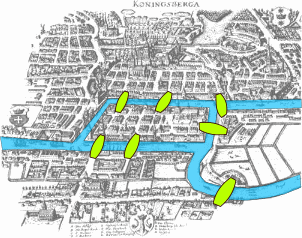
\includegraphics[width=\linewidth]{konigsberg_bridges}
    \caption{}\label{fig:konigsberg:map}
  \end{subfigure}
  \begin{subfigure}{.45\linewidth}
    \centering
    \begin{tikzpicture}
  [solmu/.style={circle,
    draw=black,
    inner sep=0pt,
    minimum size=7mm,
    node distance=5mm},
  spacer/.style={circle,
    minimum size=7mm,
    node distance=5mm}]
  \node[solmu](v1){};
  \node[spacer](s1)[right=of v1]{};
  \node[solmu](v2)[above=of s1]{};
  \node[solmu](v3)[below=of s1]{};
  \node[spacer](s2)[right=of s1]{};
  \node[solmu](v4)[right=of s2]{};
  \draw (v1) to [out=90, in=180] (v2);
  \draw (v1) to [out=10, in=270] (v2);
  \draw (v1) to (v4);
  \draw (v1) to [out=350, in=90] (v3);
  \draw (v1) to [out=270, in=180] (v3);
  \draw (v2) to (v4);
  \draw (v3) to (v4);
\end{tikzpicture}

    \caption{}\label{fig:konigsberg:tikz}
  \end{subfigure}
  \caption[Königsberg 1700-luvulla]{\subref{fig:konigsberg:map}) Königsberg 1700-luvulla, sillat vihreällä. \subref{fig:konigsberg:tikz}) Königsbergin sillat verkkona. Kuva \subref{fig:konigsberg:map}: Wikimedia Commons/Bogdan Giuşcă (CC BY-SA 3.0, \url{https://commons.wikimedia.org/wiki/File:Konigsberg_bridges.png}).}
  \label{fig:konigsberg}
\end{figure}

\section{Ongelman määrittely ja analyysi}
\label{sec:konigsberg_def}

Königbergin siltaongelma on seuraava:

\begin{problem}[Königsbergin siltaongelma]
  \label{prob:konigsberg}
  Onko Königsbergin kaupungissa sellaista kävelyreittiä, joka ylittää jokaisen sillan täsmälleen kerran. Joen ylittäminen muutoin kuin siltoja pitkin on kielletty. 
\end{problem}

\citet{euler36solutio} esitti ongelman abstraktina verkkoteorian ongelmana, missä saaret ja mantereet ovat solmuja ja sillat kaaria solmujen välillä (kuva~\ref{fig:konigsberg:tikz}). Hän osoitti, että ongelmaan ei ole ratkaisua. Nykytermein Königsbergin siltaongelman ratkaisu olisi \emph{Eulerin kulku} \engl{Euler(ian) path}, eli verkon polku joka kulkee jokaisen kaaren yli täsmälleen kerran. Eulerin tulos esitetään nykyään seuraavassa muodossa:

\begin{theorem}
  \label{thm:euler_path}
  Verkossa $G= (V, E)$ on Eulerin kulku jos ja vain jos verkossa on kaksi tai ei yhtään sellaista solmua, joiden aste on pariton.
\end{theorem}

Mikäli kulun täytyy palata takaisin alkusolmuun, puhutaan \emph{Eulerin kierroksesta}. Verkossa on Eulerin kierros jos ja vain jos siinä ei ole yhtään paritonasteista solmua.

\section{Eulerin kierroksen löytävä algoritmi}
\label{sec:euler_circuit_algo}

\citet{hierholzer73ueber} esitti tehokkaan algoritmin Eulerin kierron löytämiseksi. Algoritmi tekee mielivaltaisia kierroksia verkossa ja yhdistää niitä toisiinsa. Lopputulos tuottaa aina Eulerin kierroksen, sillä jokaisen solmun aste on aina parillinen. Algoritmi on esitetty pseudokoodina algoritmissa~\ref{alg:hierholzer}.

\begin{algorithm}[tb]
  \DontPrintSemicolon
  \SetKwInOut{Input}{syöte}\SetKwInOut{Output}{tulos}
  \SetKwProg{Fn}{function}{ }{end}
  \SetKwFunction{TeeKierros}{TeeKierros}
  \Input{Suuntaamaton verkko $G=(V, E)$ jonka jokaisen solmun aste on parillinen}
  \Output{Eulerin kierros $p$}
  \BlankLine
  $u \gets \text{mielivaltainen $V$:n solmu}$\;
  $(p, E') \gets $ \TeeKierros{$u, (V, E)$} \label{alg:hierholzer:kierrosi}\;
  \While{$E'\neq \emptyset$}{
    $u\gets \text{$p$:n mielivaltainen solmu jonka aste on $>1$ $E'$:ssa}$ \;
    $(q, E') \gets $ \TeeKierros{$u, (V, E')$} \;
    liitä polku $q$ polkuun $p$ \;
  }
  \Return{$p$}
  \BlankLine
  \Fn{TeeKierros(solmu $u$, kaaret $E$)}{
    $v\gets u$ \;
    $p\gets (u)$ \;
    \Repeat{$v = u$}{
      $w\gets \text{$v$:n mielivaltainen naapuri}$ \;
      poista kaari $\{v, w\}$ $E$:stä \;
      lisää solmu $w$ polkuun $p$ \;
      $v\gets w$ \;
    }
    \Return{$(p, E)$}
  }
  \caption{Hierholzerin algoritmi Eulerin kierroksen löytämiseksi.\label{alg:hierholzer}}
\end{algorithm}

Apufunktio \texttt{TeeKierros} tekee mielivaltaisen kierroksen alkaen solmusta $u$ ja käyttäen $E$:n kaaria. Tuloksena se palauttaa kierroksen $p$ ja kaarijoukon $E$ josta on poistettu $p$:n kaaret. Ensimmäinen kierros, rivillä~\ref{alg:hierholzer:kierrosi}, ei vielä välttämättä käytä kaikkia verkon kaaria. Niinpä apufunktiota kutsutaan toistuvasti satunnaisesta solmusta kunnes verkossa ei ole enää solmuja. 

Käyttämällä sopivia tietorakenteita, algoritmi~\ref{alg:hierholzer} voidaan toteuttaa lineaarisessa ajassa kaarten lukumäärän suhteen, $O(\abs{E})$.

% \texttt{ABCDEFGHIJKLMNOPQRSTUVWXYZÅÄÖ}\\
% \texttt{abcdefghijklmnopqrstuvwxyzåäö}\\
% \texttt{1234567890 .;-!?€}

% \textbf{\texttt{ABCDEFGHIJKLMNOPQRSTUVWXYZÅÄÖ}\\
% \texttt{abcdefghijklmnopqrstuvwxyzåäö}\\
% \texttt{1234567890 .;-!?€}}

% \setmonofont[StylisticSet=1]{Inconsolatazi4}
% \texttt{ABCDEFGHIJKLMNOPQRSTUVWXYZÅÄÖ}\\
% \texttt{abcdefghijklmnopqrstuvwxyzåäö}\\
% \texttt{1234567890 .;-!?€}

% \textbf{\texttt{ABCDEFGHIJKLMNOPQRSTUVWXYZÅÄÖ}\\
% \texttt{abcdefghijklmnopqrstuvwxyzåäö}\\
% \texttt{1234567890 .;-!?€}}


% Apufunktio \texttt{TeeKierros} tekee mielivaltaisen kierroksen alkaen solmusta $u$ ja käyttäen $E$:n kaaria.


\part{Joitain ohjeita \LaTeX{in} käyttöön}

\chapter{Johdanto}
\label{cha:latex:johdanto}

Tässä luvussa käydään läpi \LaTeX{in} käyttöä \uefcsthesis-luokan kanssa. Luku ei ole yleinen \LaTeX-käyttöohje, muttei myöskään yksityiskohtainen ohje \uefcsthesis-luokan käyttöön. Luokan ohje on tiedostossa uefcsthesis.pdf, joka sisältyy luokan dokumentaatiopakettiin.

Luvun alussa käydään läpi, kuinka tiedostoon täytetään tarvittava rakenne ja metadata. Tämän jälkeen, luvussa~\ref{cha:latex:tyonkulku}, käydään läpi erilaisia tapoja kääntää \LaTeX-tiedostoja sekä siihen liittyviä asioita, joita tulee ottaa huomioon \uefcsthesis-luokkaa käytettäessä. 

\chapter{Tiedoston rakenne}
\label{cha:latex:rakenne}

Kaikki \uefcsthesis-luokalla tehtävät opinnäytetyöt seuraavat samaa perusrakennetta. Ensimmäinen rivi on 
\begin{verbatim}
\documentclass[<optiot>]{uefcsthesis}
\end{verbatim}
missä \verb|<optiot>| ovat luokan optiota. Tyypillisimmät optiot käydään läpi luvussa~\ref{sec:latex:optiot}. Jos optioita ei anneta, luokka tekee suomenkielisen \progradututkielma{n}. 

Luokan määrittelevän käskyn \verb|\documentclass| jälkeen tulevat tyypillisesti käyttäjän itsensä \verb|\usepackage|-komennoilla lataamat paketit. Pakettien jälkeen tulevat tavallisesti käyttäjän omat komennot \verb|\newcommand|-komennolla määriteltynä, sekä muut mahdolliset \LaTeX{n} toimintaan vaikuttavat komennot (esim. ladattujen pakettien konfiguraatiokomennot).

Tämän jälkeen tulee työn metadata, kuten otsikko (komennolla \verb|\title|), tekijän nimi (komennolla \verb|\author|), ohjaajan nimi (tai ohjaajien nimet) ja niin edelleen. Näiden tietojen täyttämisestä kerrotaan enemmän luvussa~\ref{sec:latex:metadata}. Varsinainen dokumentti alkaa komennolla \verb|\begin{document}| ja loppuu komentoon \verb|\end{document}|.

Ensimmäinen komento varsinaisessa dokumentissa on
\begin{verbatim}
\maketitle
\end{verbatim}
joka tuottaa tutkielman kansisivun. Tämän jälkeen tulee tiivistelmäsivu, joka tuotetaan komentoparilla \verb|\begin{abstract}| ja \verb|\end{abstract}|. Näistä kerrotaan enemmän luvussa~\ref{sec:latex:frontmatter}.

Tiivistelmäsivujen jälkeen dokumentissa täytyy tulla komento
\begin{verbatim}
\frontmatter
\end{verbatim}
Tämä komento kertoo \LaTeX:ille, että seuraaville sivuille tulee laittaa sivunumero roomalaisin numeroin. Komento \verb|\tableofcontents| ainut pakollinen sisältö ennen komentoa \verb|\mainmatter|, joka taas kertoo \LaTeX:ille, että tästä eteenpäin kyseessä on varsinainen dokumentin tekstiosa, jossa sivunumerot ovat normaaleilla numeroilla.

Varsinaisen osan lopussa tulee sisällysluettelo. Se voidaan lisätä joko komennolla \verb|\bibliography| tai komennolla \verb|\printbibliography|, riippuen siitä, käytetäänkö Bib\LaTeX- vai Bib\TeX-ohjelmaa. Lopussa täytyy olla \verb|\backmatter| komento, joka kertoo \LaTeX{ille}, missä viimeinen varsinaisen materiaalin sivu on. Tämän jälkeen voi vielä tulla liitteitä ennen \verb|\end{document}|-komentoa.

Minimaalinen esimerkki luokan käytöstä on näytetty listauksessa~\ref{lst:minimal}. Tämä esimerkki tulee \uefcsthesis-paketin mukana tiedostossa nimeltä \texttt{minimal\_classic.fi.tex}.


\lstset{language=[AlLaTeX]TeX,
basicstyle=\small,
columns=fullflexible,
morekeywords={\addbibresource, \city, \firstsupervisor, \secondsupervisor, \keywords, \maketitle, \frontmatter, \tableofcontents, \mainmatter, \chapter, \citep, \citet, \printbibliography, \backmatter, \sep, \Title, \Author, \Keywords, \Subject, \Publisher}
}

\lstinputlisting[
float=tbp,
caption={Minimaalinen \texttt{.tex}-tiedosto \uefcsthesis-luokan käyttämiseksi.},
label=lst:minimal,
frame=lines,
firstline=34,
lastline=78,
]{minimal_classic.fi.tex}


\section{Luokan optiot}
\label{sec:latex:optiot}

Luokan \uefcsthesis tärkeimmät optiot valitsevat opinnäytetyön tyypin (\progradututkielma vai kandidaatintutkielma) ja kielen (suomi vai englanti). Sen lisäksi luokalle voi antaa joukon muita optioita, joilla voidaan esim.\ tuottaa PDF/A-muotoisia tiedostoja. Tärkeimmät optiot on listattu taulussa~\ref{tab:latex:optiot}. Kaikki optiot löytyvät luokan käyttöohjeesta.

\begin{table}[tbp]
  \small
  \centering
  \caption{Luokan \uefcsthesis tärkeimmät optiot. Samassa ryhmässä olevat optiot ovat toisensa poissulkevia. Ylin vaihtoehto kustakin ryhmästä on oletusarvo.}
  \label{tab:latex:optiot}
  \begin{tabularx}{\linewidth}{@{}p{.25\linewidth}>{\ttfamily}lX@{}}
    \toprule
    Ryhmä & \textrm{Optio} & \multicolumn{1}{c}{Kuvaus} \\
    \midrule
    Työn tyyppi & mscthesis & Asettaa tyypiksi \progradututkielma{n} \\
    & gradu & Sama kuin yllä \\
    & bscthesis & Asettaan tyypiksi kandidaatintutkielman \\
    & kandi & Sama kuin yllä \\
    Kieli & finnish & Asettaa kieleksi suomen \\
    & english & Asettaa kieleksi amerikanenglannin \\
    & british & Asettaa kieleksi brittienglannin \\
    Kielten tuki & polyglossia & Käyttää kielten tukemiseen \texttt{polyglossia}-pakettia \texttt{babel}-paketin sijasta \\
    Viimeistely & final & Tuottaa viimeistellyn dokumentin \\
    & draft & Tuottaa luonnostasoisen dokumentin \\
    Viiteohjelmisto & bibtex & Käyttää Bib\TeX-ohjelmistoa viitteiden hallintaan \\
    & biblatex & Käyttää Bib\LaTeX-pakettia viitteiden hallintaan \texttt{biber}-ohjelmiston kanssa \\
    PDF/A & nopdfa & Ei luo PDF/A-tyyppistä tiedostoa \\
    & pdfa & Luo PDF/A-tyyppisen tiedoston \\
    \bottomrule
  \end{tabularx}
\end{table}

\paragraph{Työn tyyppi.}
Työn tyypiksi voidaan asettaa joko \progradututkielma tai kandidaatintutkielma. Pro gradu asetetaan antamalla joko \texttt{mscthesis}- tai \texttt{gradu}-optio. Nämä optiot käyttäytyvät täysin samoin, eivätkä esim. muuta kieltä. Kandidaatintutkielma asetetaan tyypiksi optioilla \texttt{bscthesis} tai \texttt{kandi}. Myöskään nämä eivät muuta kieltä. Kandidaatin- ja \progradututkielma{t} asetellaan hieman eri tavalla, minkä lisäksi tyyppi vaikuttaa nimiö- ja tiivistelmäsivujen sisältöön sekä PDF-tiedoston metadataan. Mikäli mitään tyyppiä ei anneta, on oletuksena \progradututkielma.

\paragraph{Kieli ja kielen tuki.}

Työn kieleksi voidaan valita joko suomi (optio \texttt{finnish}), amerikanenglanti (option \texttt{english}) tai brittienglanti (optio \texttt{british}). Kieli vaikuttaa -- luonnollisesti -- sekä kaikkiin luokan tuottamiin teksteihin että tavutukseen ja lähdeluettelon sisältöön. Oikean kielen asettaminen on ehdottoman tärkeää. Ole\-tuk\-se\-na kieli on suomi. Perinteisesti \LaTeX{issa} on käytetty \texttt{babel}-ohjelmistoa tavuttamiseen ja muuhun erikielisten dokumenttien tukemiseen, mutta uudempien \LaTeX-ohjelmistojen (kuten Lua\LaTeX) kanssa \texttt{polyglossia}-paketti toimii monesti paremmin. Sitä (ja Lua\LaTeX{ia} tai Xe\LaTeX{ia}) suositellaan käytettäväksi varsinkin, jos työ sisältää muitakin kieliä kuin suomea tai englantia (esim.\ venäjää tai japania). 

\paragraph{Viimeistely.}

Luokka tukee \LaTeX{in} standardeja \texttt{draft} ja \texttt{final} optioita. Luonnos (\texttt{draft}) ei lataa kuvia ja merkitsee marginaalin rivit, jotka ovat ylipitkiä. Jotkut paketit huomioivat myös \texttt{draft}-option ja muuttavat toimintaansa sen mukaan. Ole\-tuk\-se\-na luokka käyttää \texttt{final}-optiota, joka tuottaa normaalin lopputuloksen.

\paragraph{Viiteohjelmisto.}

Perinteisesti \LaTeX{in} lähdeviittausten hallintaan käytetään Bib\TeX-oh\-jel\-mis\-toa. Tämä on myös \uefcsthesis-luokan oletus. Käytettäessä Bib\TeX-oh\-jel\-mis\-toa, \uefcsthesis lataa \texttt{apacite}-paketin,\!\footnote{\url{https://ctan.org/pkg/apacite}, viitattu 23.12.2018.} joka vastaa lähdeviittausten muotoilusta ja viittauslistan muotoilusta. Toinen vaihtoehto on käyttää \texttt{biblatex}-optiota, joka lataa Bib\LaTeX-paketin\footnote{\url{https://ctan.org/pkg/biblatex}, viitattu 23.12.2018} ja edellyttää, että viittauslistan tekemiseen käytetään \texttt{biber}-ohjelmaa. Bib\LaTeX{} tukee Unicode-merkistöä paremmin kuin Bib\TeX, ja tarjoaa monipuolisemmat ominaisuudet lähdeviitteiden hallintaan, mutta paketti edellyttää samalla uudempaa \LaTeX-ympäristöä. Lähdeviitteiden teosta kerrotaan enemmän luvussa~\ref{sec:latex:mainmatter_backmatter} ja \texttt{biblatex} sekä \texttt{biber} ohjelmien käytöstä luvussa~\ref{cha:latex:tyonkulku}.

\paragraph{PDF/A-muotoiset tiedostot.}

Itä-Suomen yliopiston ohjeiden mukaan \progradututkielma{t} tulee palauttaa PDF/A-muodossa. Kun \uefcsthesis-luokalle annetaan \texttt{pdfa} optio, se tuottaa PDF/A-1b-muotoisen PDF-tiedoston. Tiedoston tuottaminen edellyttää oikeanlaisen metadatatiedoston olemassaoloa. Oletuksena (optio \texttt{nopdfa}) \uefcsthesis tekee normaalin PDF-tiedoston, jota voi mm.\ editoida ja kommentoida.

\begin{tikzpicture}[baseline]
  \node[huombox] (miktexbiber) {
    \begin{minipage}{0.9\textwidth}
      PDF/A-tiedostojen luominen on vielä beta-vaiheessa, eikä se välttämättä toimi. \LaTeX:n tuottaman PDF-tiedoston voi kääntää PDF/A-muotoon esim. Adoben Acrobat Pro -ohjelmalla.
    \end{minipage}
  };
  \node[huomtitle,right=10pt] at (miktexbiber.north west) {Huom!};
\end{tikzpicture}

\section{Työn metatiedot}
\label{sec:latex:metadata}

Työn metatiedot annetaan \LaTeX-dokumentin johdanto-osassa \engl{preamble}, eli ennen \verb+\begin{document}+-komentoa. Metatiedot annetaan niitä vastaavien makrojen parametreina. Esimerkiksi kirjoittajan nimi annetaan makrolla \texttt{author} muodossa \verb+\author{Etunimi}{Sukunimi}+. Kaikki metadatan syöttämiseen liittyvät makrot on listattu taulukossa~\ref{tab:metadata_macros}.

\begin{table}
  \centering
  \caption{Makrot opinnäytetyön metadatan syöttämiseksi.}
  \label{tab:metadata_macros}
  \small
  \begin{tabular}{
    @{}
    l
    >{\ttfamily\textbackslash}l
    >{\ttfamily\textbackslash}l
    @{}
    }
    \toprule
    Tietue & \multicolumn{1}{c}{Makro} & \multicolumn{1}{c}{Esimerkki} \\
    \midrule
    Otsikko  & title & title\{Otsikko\} \\
    Aliotsikko & subtitle & subtitle\{Aliotsikko\} \\
    Kirjoittaja & author & author\{Etunimi\}\{Sukunimi\} \\
    Päivämäärä & date & date\{Tammikuu 2019\} \\
    Kaupunki & city & city\{Kuopio\} \\
    Pääohjaaja & firstsupervisor & firstsupervisor\{Etu Suku\} \\
    Toinen ohjaaja & secondsupervisor & secondsupervisor\{Etu Suku\} \\
    Avainsanat & keywords & keywords\{asana1\textbackslash sep asana2\} \\
    ACM CCS -luokka & ccsdesc & ccsdesc[500]\{Some Class\} \\
    Liitteiden lukumäärä & numberofappendices & numberofappendices\{2\} \\
    Liitteiden sivumäärä & appendixpagecount & appendixpagecount\{20\} \\
    \bottomrule
  \end{tabular}
\end{table}



\paragraph{Otsikko.}
Työn otsikko annetaan \texttt{title}-makrolla. Jos työllä on aliotsikko, se annetaan \texttt{subtitle}-makrolla. Suomenkielisillä opinnäytetöillä tulee olla otsikko (ja tiivistelmäsivu) myös englanniksi. Nämä annetaan lisäämällä valinnainen parametri, joka kertoo otsikon kielen, esim:
\begin{verbatim}
\title[english]{Title in English} 
\subtitle[english]{Subtitle in English}
\end{verbatim}

\paragraph{Kirjoittaja.}
Toisin kuin useimmissa \LaTeX-tyyleissä, \verb+\author+-makro saa kaksi parametria. Mahdolliset muiden etunimien alkukirjaimet kirjoitetaan etunimen kanssa  ensimmäiseen parametriin, esim. \verb+\author{John R. R.}{Tolkien}+.

\paragraph{Päivämäärä ja paikka.}
Työn valmistumiskuukausi ja -vuosi kirjoitetaan \texttt{date}-makron syötteeksi. Englanninkieliset päivämäärät voi vastaavasti täyttää lisäämällä valinnaisen kieliparametrin:
\begin{verbatim}
\date[english]{January 2019}
\end{verbatim}
Työn valmistumiskaupunki annetaan makrolla \texttt{city}. Kaupungin nimeä ei tarvitse kirjoittaa erikseen englanniksi, mutta mikäli työhön halutaan tiivistelmäsivu kielellä, jolla kaupungin nimi eroaa suomenkielisestä, sen voi antaa vastaavalla tavalla määrittelemällä kielen valinnaisessa parametrissa (erikielisten tiivistelmäsivujen tekeminen selitetään luvussa~\ref{sec:latex:frontmatter}).

\paragraph{Ohjaajat.}
Tyypillisesti opinnäytetöillä on yksi tai kaksi ohjaajaa/tarkastajaa. Heidän nimensä kirjoitetaan \texttt{firstsupervisor}- ja \texttt{secondsupervisor}-makrojen parametreiksi. Mikäli työllä on useampi kuin kaksi ohjaajaa, kirjoitetaan muiden kuin viimeisen ohjaajan nimet \texttt{firstsupervisor}-makron parametriin pilkuilla erotettuna; viimeisen ohjaajan nimi kirjoitetaan tavalliseen tapaan \texttt{secondsupervisor}-makron parametriksi.

\paragraph{Avainsanat ja CCS-luokittelu.}
Avainsanat annetaan \texttt{keywords}-makrolla. Avainsanat erotellaan toisistaan \texttt{sep}-makrolla; erotinmerkki muuttuu käyttötarkoituksesta riippuen, ja \uefcsthesis-luokka muuttaa \texttt{sep}-makron määritelmää tarpeen mukaan. Englanninkieliset avainsanat syötetään tavalliseen tapaan antamalla \texttt{keywords}-makrolle valinnainen kieliparametri.

Tutkielmat tulee luokitella myös ACM:n vuoden 2012 luokittelujärjestelmällä.\footnote{ACM 2012 Computing Classification System (CCS), \url{https://www.acm.org/publications/class-2012}, viitattu 1.1.2019} Oman luokittelun tekemiseksi kannattaa käyttää ACM:n web-pohjaista ohjelmaa osoitteessa \url{https://dl.acm.org/ccs/ccs.cfm} (viitattu 1.1.2019). Opinnäytetyön luokat valitaan kulkemalla luokittelupuussa ylätason luokista alemmas. Kun haluttu luokka on löytynyt, lisätään se valittuihin luokkiin vasemmalla olevasta \textquote{Assing This CCS Concept}-linkistä (kuva~\ref{fig:latex:ccs}, punainen nuoli). Tämä avaa pop-up-ikkunan, jossa pitää valita luokan merkittävyys. Jos tämän jälkeen halutaan lisätä uusia luokkia, voidaan valita \textquote{continue}-linkki. Jos taas halutaan kopioida CCS-luokittelu tutkielmaan, valitaan \textquote{view CCS TeX Code}-linkki (kuva~\ref{fig:latex:ccs}, violetti nuoli). Tämä näyttää luokittelun \LaTeX-koodin. Koko koodia ei tarvitse kopioida: XML-koodin voi jättää pois, mutta \texttt{ccsdesc}-makro(t) argumentteineen pitää kopioida.

\begin{figure}[tbp]
  \centering
  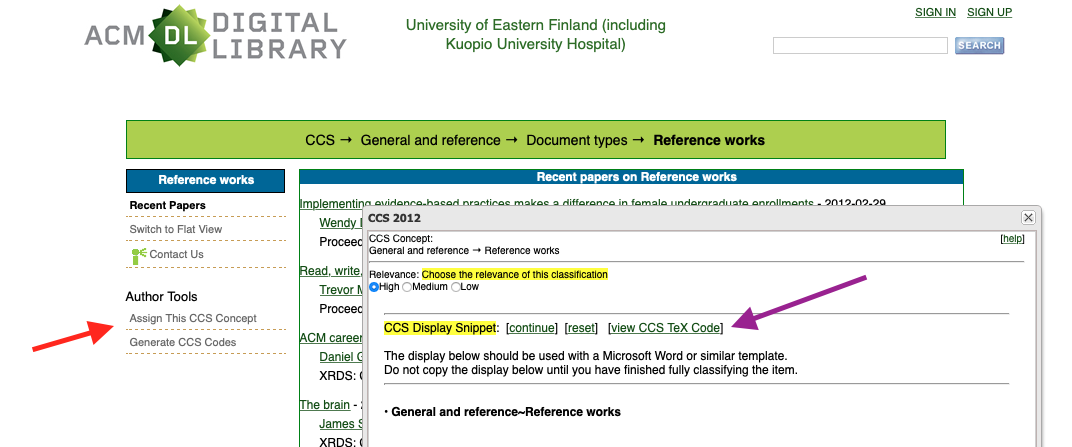
\includegraphics[height=6cm]{ccs_overview}\\[1em]
  \rule{\textwidth}{0.4pt}\\[1em]
  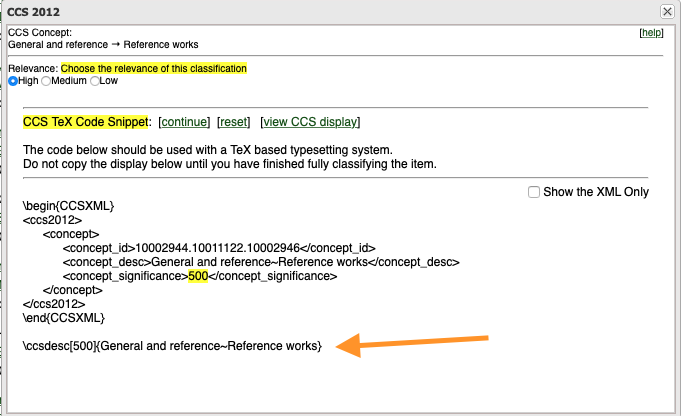
\includegraphics[height=5cm]{ccs_latex_code}
  \caption[Esimerkki ACM:n CCS:n käytöstä]{Esimerkki ACM:n CCS-luokittelijaohjelman käytöstä. Yllä punainen nuoli osoittaa linkin, josta luokka valitaan ja violetti nuoli osoittaa linkin, josta näkee \LaTeX-koodin. Alla oranssi nuoli osoittaa sen kohdan \LaTeX-koodia, joka tulee kopioida tutkielman metatietoihin. }
  \label{fig:latex:ccs}
\end{figure}

\paragraph{Liitteet.}
Mikäli tutkielmaan kuuluu liitteitä, niiden luku- ja sivumäärä pitää kertoa erikseen. Tämä mahdollistaa myös sellaisten liitteiden lisäämisen lopulliseen tutkielmaan, jotka eivät ole osa \LaTeX-tiedostoa. Liitteiden lukumäärä annetaan \texttt{numberofappendices}-makrolla ja niiden yhteenlaskettu sivumäärä \texttt{appendixpagecount}-makrolla. Mikäli tutkielmaan ei kuulu liitteitä, näitä makroja ei tarvitse käyttää.

\section{Otsikkosivu, tiivistelmäsivut ja muut sivut ennen varsinaista tekstiä}
\label{sec:latex:frontmatter}


Työn otsikko- ja tiivistelmäsivujen tiedot annetaan pääosin edellisessä luvussa kuvattujen makrojen avulla. Kun työn metatiedot on määritelty, aloitetaan varsinainen dokumentti \verb+\begin{document}+-komennolla. Otsikkosivu tehdään makrolla \verb+\maketitle+. Makro ei saa argumentteja.

  Otsikkosivun jälkeen tiivistelmä kirjoitetaan \texttt{abstract}-ympäristön sisään. Tähän kirjoitetaan pelkästään tiivistelmän teksti; avainsanat ja luokittelu on määritelty jo aiemmin. Ympäristö tuottaa myös tiivistelmäsivun dokumentin pääkielellä. Suomenkielisissä tutkielmissa tulee olla myös englanninkielinen tiivistelmä. Se kirjoitetaan uuden \texttt{abstract}-ympäristön sisään, jolle on annettu valinnainen kieliargumentti \textquote{english}:
\begin{verbatim}
\begin{abstract}[english]
  Abstract in English.
\end{abstract}
\end{verbatim}

  Englanninkielinen tiivistelmäsivu edellyttää, että työn otsikko ja päivämäärä on määritelty myös englanniksi metatiedoissa.
  
  Tiivistelmäsivujen jälkeen \emph{pitää} tulla komento \verb+\frontmatter+. Tämä komento kertoo, että seuraavat sivut numeroidaan roomalaisin numeroin ja ne eivät kuulu varsinaiseen tekstiin. Jokaisessa tutkielmassa ainakin sisällysluettelo on tällainen sivu. Sisällysluettelo tehdään \verb+tableofcontents+-komennolla. Muita mahdollisia osia ovat esipuhe (\texttt{preface}-ympäristö) ja kiitokset (\texttt{acknowledgements}-ympäristö); useimmissa tutkielmissa on vain toinen näistä osista.

\section{Leipäteksti, viitteet ja liitteet}
\label{sec:latex:mainmatter_backmatter}

Tutkielman varsinainen sisältö aloitetaan \verb+\mainmatter+-komennolla. Tämä komento on myös pakollinen; ilman sitä sivunumerointi jää käyttämään roomalaisia numeroita.

Tutkielman sisältö kannattaa jakaa useaan tiedostoon esimerkiksi jakamalla jokaisen luvun omaan tiedostoonsa. Tiedostot saa liitettyä osaksi dokumenttia \verb+\input+-komennolla. Päätiedostossa leipätekstin sijasta voi siis olla pelkkiä \verb+\input+-komentoja:
\begin{verbatim}
\mainmatter
\input{johdanto}
\input{kirjallisuuskatsaus}
\input{menetelmä}
\input{kokeet}
\input{loppuyhteenveto}
\end{verbatim}

Sisällytetyt tiedostot (esim. \texttt{johdanto.tex}) voivat sisällyttää uusia tiedostoja.

\paragraph{Väliotsikot.}
Opinnäytetöissä on tyypillisesti kahden tason väliotsikoita: lukuja ja alilukuja. Luvut tehdään \uefcsthesis-luokassa \verb+\chapter+-komennolla. Pro gradu \nobreakdash-tutkielmissa \uefcsthesis{} latoo luvut alkamaan omalta sivultaan; kandidaatintutkielmissa ne alkavat heti edellisen sivun lopusta. Aliluvut tehdään \verb+\section+-komennolla. Tarvittaessa on mahdollista tehdä myös matalamman tason numeroituja lukuja käyttämällä \verb+\subsection+-komentoa, mutta tavallisesti näin hienojakoinen jaottelu viittaa ongelmiin tutkielman rakenteessa. Yleensä onkin parempi käyttää numeroimattomia osia esimerkiksi \verb+\subsubsection+- tai \verb+\paragraph+-komennoilla.

Kaikille väliotsikoille kannattaa antaa nimiö \verb+\label+-komennolla, vaikkei niihin juuri sillä hetkellä aiokkaan viitata. Näin viittauksen voi lisätä myöhemmin tarvitsematta palata lisäämään nimiötä. Sama toki koskee myös muita viitattavia \LaTeX-elementtejä, kuten kuvia, tauluja, lauseita, lemmoja ja yhtälöitä.

\paragraph{Viitteet.}
\LaTeX{issa} viitteitä hallitaan joko Bib\TeX- tai \texttt{biber}-ohjelmalla. Nämä lukevat tekstissä olevat viittauskomennot (esim. \verb+\citep+ ja \verb+\citet+) ja erillisen lähdetietokannan (tiedostopääte \texttt{.bib}) ja rakentavat lähdeluettelon sekä korvaavat viittauskomennot varsinaisilla viitteillä. 

Oletuksena \uefcsthesis käyttää APA-tyylin viittauksia, joissa viittaukset tekstissä ovat muotoa \textquote{(tekijä/t, vuosi)}. Jos tekijöiden nimiä tarvitaan ympäröivässä virkkeessä, viittaus voi olla muotoa \textquote{tekijä/t (vuosi)}. Sulkeiden sisällä oleva viittaus tehdään \verb+\citep+-komennolla (\texttt{p} = parenthesis) ja viittaus, jossa tekijöiden nimet ovat sulkeiden ulkopuolella, tehdään \verb+\citet+-komennolla (\texttt{t} = text). Esimerkiksi:
\begin{displayquote}
  \verb+\citep+: Königsbergin siltaongelmaan ei ole ratkaisua \citep{euler36solutio}.\\
  \verb+\citet+: \citet{euler36solutio} todisti, ettei Königsbergin siltaongelmaan ole ratkaisua.
\end{displayquote}

Useampi viite voidaan kirjoittaa saman komennon sisään pilkuilla erotettuna ja \uefcsthesis järjestää ne tekijöiden nimien ja vuosien mukaan. Viittauskomentoina käytetään \texttt{natbib}-paketin komentoja \citep{natbib}, ja paketin dokumentaatioon kannattaa perehtyä.\footnote{Paketin \textquote{cheat sheet} on hyvä tiivistelmä: \url{https://www.texlive.info/CTAN/macros/latex/contrib/natbib/natnotes.pdf} (viitattu 2.10.2019)} Kirjoittajien nimien taivuttaminen sijamuotoihin (esim. \textquote{Eulerin (1741) mukaan}) ei kuitenkaan ole mahdollista, muutoin kuin kirjoittamalla tekijöiden nimet itse. Helpointa lienee välttää sellaiset lauserakenteet, joissa tarvittaisiin nimien sijamuotoja. \LaTeX{in} perinteistä \verb+\cite+-komentoa ei kannata käyttää -- vaikka se toimiikin -- sillä siitä ei käy ilmi, halutaanko tekijöiden nimet sulkeiden sisään vai ei (\texttt{natbib}-paketti asettaa \verb+\cite+=\verb+\citet+). Bib\LaTeX-pakettia ja \texttt{biber}-ohjelmaa käytettäessä voidaan myös käyttää \texttt{natbib}-viittauskomentoja. Vaihtoehtoisesti voidaan käyttää myös Bib\LaTeX-paketin omia viittauskomentoja.\footnote{Paketin Bib\LaTeX{} \textquote{cheat sheet} on osoitteessa \url{http://tug.ctan.org/info/biblatex-cheatsheet/biblatex-cheatsheet.pdf}, viitattu 3.10.2019.}

Itse lähdeluettelo lisätään tutkielman loppuun viimeisenä osana ennen pakollista \verb+\backmatter+-komentoa. Käytettäessä Bib\TeX-ohjelmaa lähdeluettelo lisätään \verb+\bibliography+-komennolla, jonka argumentiksi tulee lähdetietokantatiedoston nimi. Käytettäessä \texttt{biber}-ohjelmaa, lähdetietokannan nimi annetaan ennen \verb+\begin{document}+-komentoa käyttämällä \verb+\addbibresource+-komentoa ja lähdeluettelon paikka osoitetaan komennolla
\begin{verbatim}
\printbibliography[heading=bibintoc]
\end{verbatim}
  
\paragraph{Liitteet.}
Mikäli tutkielmaan halutaan lisätä liitteitä, ne tulee laittaa \verb+\backmatter+-komennon jälkeen. Liitteiden luku- ja sivumäärä tulee myös kertoa dokumentin johdannossa (ks. luku~\ref{sec:latex:metadata}). Mahdollisia liitteitä ovat esimerkiksi listaukset tutkielmassa olevista kuvista, taulukoista tai algoritmeista, työssä käytettyjen tai kehitettyjen algoritmien täydelliset ohjelmalistaukset tai testien täydelliset tulokset. 

Kaikki \LaTeX{issa} tehtävät liitteet kirjoitetaan yhden \texttt{appendices}
-ympäristön sisään. Liitteet otsikoidaan \texttt{chapter}-tason otsikoilla. Jos työhön halutaan liittää liitteitä, jotka eivät ole tehty \LaTeX{illa}, on käytössä seuraavia vaihtoehtoja:
\begin{enumerate}
\item PDF-muodossa olevat lisättävät liitteet voi sisällyttää suoraan dokumenttiin:
\begin{verbatim}
\begin{appendices}
  \chapter{Ulkoinen liite}
  \includegraphics[pages={1-}]{liite.pdf}
\end{appendices}
\end{verbatim}
\item Liitteen otsikkosivun voi tehdä \LaTeX{issa} ja varsinaisen sisällön voi liittää tutkielman PDF:n loppuun (esim. Linuxissa \texttt{pdfcat}-komennolla tai käyttäen Acrobat Pro -ohjelmaa tai MacOS:n Esikatselu-ohjelmaa)
\item Jos liitteessä on jo oikein numeroitu otsikko, sen voi lisätä suoraan tutkielman PDF:n loppuun. Tällöin liitteen otsikko ei tule näkyviin sisällysluetteloon. Jos liitteitä on vain yksi, voidaan dokumenttiin lisätä seuraavat rivit:
\begin{verbatim}
\begin{appendices}
  \addcontentsline{toc}{chapter}{LIITTEEN OTSIKKO}
\end{appendices}
\end{verbatim}
  Mikäli liitteitä on useampia, korvataan \verb+\addcontentsline+-rivi seuraavilla:\\
  \verb+\addcontentsline{toc}{chapter}+\\
  \verb+{\numberline {X}LIITTEEN OTSIKKO}+,\\
  missä X on liitteen järjestyksen osoittava kirjain.
\end{enumerate}

Käytettyjen kuvien ja taulukkojen listaukset on mahdollista lisätä lisäämällä komennot \verb+\listoffigures+ ja \verb+\listoftables+ \texttt{appendices}-ympäristön sisään. Esitetyistä pseudokoodeista ja ohjelmalistauksista on myös mahdollista lisätä oma listauksensa, mutta tarkat komennot riippuvat käytetyistä paketeista. 

\chapter{\LaTeX-tiedostojen kääntäminen}
\label{cha:latex:tyonkulku}

% Tyyli komentorivitekstin näyttämiseen
\lstdefinestyle{cmdline}{language=bash,basicstyle=\small\ttfamily}

\LaTeX-tiedostoja voi kääntää PDF-tiedostoiksi useilla eri tavoilla ja useilla eri ohjelmilla. Seuraavassa esitellään eri käyttöjärjestelmien omia vaihtoehtoja ja huomioitavia asioita. Ensin käsitellään kuitenkin tiedostojen kääntäminen komentoriviltä, sillä se toimii kaikissa käyttöjärjestelmissä. 

\section{Komentorivi}
\label{sec:latex:komentorivi}

Useimmin käytetty ohjelma on nimeltään \texttt{pdflatex}. Komentoriviltä käytettäessä tiedoston \texttt{tiedosto.tex} kääntäminen PDF-muotoon vaatii seuraavia komentoja
\begin{lstlisting}[style=cmdline]
pdflatex tiedosto
bibtex tiedosto
pdflatex tiedosto
pdflatex tiedosto
\end{lstlisting}
Sama tiedosto pitää ajaa useamman kerran ohjelman läpi, jotta ristiinviittaukset voidaan ratkaista. Välissä \texttt{bibtex} rakentaa lähdeluettelon.

XeLaTeX ja LuaLaTeX tarjoavat joitain parannuksia \texttt{pdflatex}-ohjelmaan. Suurimmassa osassa tutkielmia nämä parannukset eivät ole oleellisia ja \texttt{pdflatex} riittää, mutta jos esimerkiksi halutaan käyttää muita fontteja kuin Times New Roman, XeLaTeX on parempi, kun taas LuaLaTeX mahdollistaa joidenkin kehittyneempien pakettien käytön esim. verkkojen automaattisessa piirtämisessä. Lisäksi XeLaTeX ja LuaLaTeX tukevat UTF-8-koodausta paremmin kuin \texttt{pdflatex}. Näitä kahta voidaan käyttää vaihtamalla \texttt{pdflatex}-komento joko \texttt{xelatex}- tai \texttt{lualatex}-komentoihin.

Käytettäessä XeLaTeXia tai LuaLaTeXia, on suositeltavaa käyttää myös \texttt{polyglossia}-pakettia suomenkielisen tavutuksen tekemiseen \texttt{babel}-paketin sijasta sekä \texttt{biber}-ohjelmaa \texttt{biblatex}-ohjelman sijasta lähdeluettelon tekemiseen.\footnote{Nämä eivät ole pakollisia, ja toisaalta \texttt{biber}-ohjelmaa voi käyttää myös \texttt{pdflatex}in kanssa.} Nämä otetaan käyttöön lisäämällä tarvittavat optiot \uefcsthesis-luokalle (ks. taulukko~\ref{tab:latex:optiot}). Käytettäessä LuaLaTeXia ja \texttt{biber}iä yllä oleva esimerkki muutettaisiin muotoon
\begin{lstlisting}[style=cmdline]
lualatex tiedosto
biber tiedosto
lualatex tiedosto
lualatex tiedosto
\end{lstlisting}

Yksittäisten komentojen kirjoittamisen sijasta voi käyttää myös  \texttt{latexmk}-ohjelmaa, joka tulee useimpien \LaTeX-asennuksien mukana. Ohjelma on kirjoitettu Perl-kielellä, joten se edellyttää Perl-tulkin. Käytettäessä \texttt{latexmk}-ohjelmaa riittää kertoa, millä \LaTeX-tulkilla tiedosto halutaan kääntää (\texttt{pdflatex}, \texttt{lualatex} vai \texttt{xelatex}). Ohjelma suorittaa tulkin tarpeeksi monta kertaa ja suorittaa myös oikean viiteohjelmiston. Esimerkiksi
\begin{lstlisting}[style=cmdline]
latexmk -pdf tiedosto
\end{lstlisting}
käyttää \texttt{pdflatex}ia ja
\begin{lstlisting}[style=cmdline]
latexmk -lualatex tiedosto
\end{lstlisting}
LuaLaTeX-ohjelmaa.

\section{Linux}
\label{sec:latex:linux}

Linuxissa \LaTeX{} on yleensä valmiiksi asennettuna. Yleisin \LaTeX-jakelupaketti on TeX Live, joka pitää sisällään kaikki ne paketit, joita \uefcsthesis tarvitsee. Vuoden 2017 tai vanhemmat TeX Live -jakelut eivät kuitenkaan välttämättä toimi. Lisätietoja TeX Livestä osoitteessa \url{https://www.tug.org/texlive/} (viitattu 3.10.2019).

Linuxille on saatavilla iso joukko \LaTeX{}-kehitysympäristöjä (IDE). Perinteiset Emacs ja vim tukevat \LaTeX{ia} erittäin hyvin ja ovatkin eräitä suosituimpia tekstieditoreita \LaTeX-tiedostojen kirjoittamiseen. Erityisesti \LaTeX{ille} suunnattuja ilmaisia IDEjä ovat mm. LyX\footnote{\url{https://www.lyx.org}, viitattu 3.10.2019}, Texmaker\footnote{\url{https://www.xm1math.net/texmaker/}, viitattu 3.10.2019} ja TeXstudio.\footnote{\url{https://www.texstudio.org}, viitattu 3.10.2019} Myös esimerkiksi Eclipse\footnote{\url{https://projects.eclipse.org/projects/science.texlipse}, viitattu 3.10.2019} ja Visual Studio Code\footnote{\url{https://marketplace.visualstudio.com/items?itemName=James-Yu.latex-workshop}, viitattu 3.10.2019} tukevat \LaTeX-editointia lisäpakettien avulla.

\section{Windows}
\label{sec:latex:windows}

Yleisin \LaTeX-jakelupaketti Windows-ympäristöissä on MiKTeX.\footnote{\url{https://miktex.org}, viitattu 3.10.2019} MiKTeXin voi asentaa yliopiston koneisiin UEF:n Software Centeristä ja esim. mikroluokkien koneisiin se on jo asennettu. MiKTeX poikkeaa TeX Live -jakelusta siinä, että MiKTeX lataa \LaTeX{in} lisäpaketteja koneelle vain, kun niitä ensimmäistä kertaa tarvitaan. Tässä vaiheessa MiKTeX saattaa ladata vanhan version paketista. On myös mahdollista, että MiKTeX lataa paketin joka tarvitsee uudemman version koneella jo olevasta paketista. Jos MiKTeX tuottaa virheilmoituksia, kuten
\begin{lstlisting}[style=cmdline]
! LaTeX Error: File `l3backend-pdfmode.def' not found.
\end{lstlisting}
kannattaa ensin päivittää kaikki MiKTeXin paketit ja yrittää kääntää dokumenttia uudelleen (jälkimmäisen ilmoituksen kohdalla kannattaa myös varmistaa, että paketti \texttt{l3backend} on ladattuna koneelle).

Moni Linuxille saatavista IDEstä toimii myös Windowsissa, kuten Texmaker ja TeXstudio (sekä tietenkin eclipse ja VS Code). TeXnicCenter\footnote{\url{http://www.texniccenter.org}, viitattu 3.10.2019} on vain Windowsilla toimiva \LaTeX-IDE. 

\begin{tikzpicture}[baseline]
\node[huombox] (miktexbiber) {
  \begin{minipage}{0.9\textwidth}
    Tällä hetkellä (6.10.2019) yliopiston MiKTeX asennus ei toimi yhdessä \texttt{biber}-ohjelman ja bib\LaTeX-paketin kanssa. Jos \uefcsthesis-luokalle antaa option \texttt{biblatex} ja lähdeluettelon yrittää luoda \texttt{biber}-ohjelmalla, tulee seuraava virheilmoitus:
    \begin{lstlisting}[style=cmdline,basicstyle=\scriptsize\ttfamily]
      ERROR - Error: Found biblatex control file version 3.6, expected version 3.5.
      This means that your biber (2.12) and biblatex (3.13a) versions are incompatible.
      See compat matrix in biblatex or biber PDF documentation.
      INFO - ERRORS: 1
    \end{lstlisting}
    Ongelma korjautuu, kunhan \texttt{biber}-ohjelmasta ja bib\LaTeX-paketista on saatavissa yhteensopivat versiot.
  \end{minipage}
};
\node[huomtitle,right=10pt] at (miktexbiber.north west) {Huom!};
\end{tikzpicture}


\section{MacOS}
\label{sec:latex:macos}

MacOS-käyttöjärjestelmän yleisin \LaTeX-jakelupaketti on MacTeX,\footnote{\url{http://www.tug.org/mactex/}, viitattu 3.10.2019} joka on TeX Liven Mac-versio. Kuten TeX Livessä, \uefcsthesis toimii ainakin vuoden 2018 MacTeXillä tai uudemmilla.

MacTeX asentaa oletuksena TeXShop-IDE:n, BibDesk-ohjelman,\footnote{\url{https://bibdesk.sourceforge.io}, viitattu 3.10.2019} jolla voi hallita Bib\TeX{in} ja Bib\LaTeX{in} viittaustietokantoja, sekä joitain muitakin apuohjelmia.  Myös suurin osa Linuxin kohdalla mainituista editoreista toimii MacOS:ssa.

\section{Online-palvelut}
\label{sec:latex:internet}

Käyttöjärjestelmästä riippumattomana vaihtoehtona voi käyttää myös online-palveluja, jotka mahdollistavat \LaTeX-dokumenttien editoinnin ja kääntämisen selaimessa. Suosituin palvelu on Overleaf,\footnote{\url{https://www.overleaf.com}, viitattu 3.10.2019} jonka käyttäminen yhden käyttäjän projekteille on ilmaista. Helpoin tapa saada \uefcsthesis toimimaan Overleafissa on kopioida \texttt{uefcsthesis.zip}-paketti sellaisenaan Overleafiin ja aloittaa opinnäytetyön kirjoittaminen muokkaamalla joko \texttt{minimal\_modern.fi.tex}- tai \texttt{minimal\_classic.fi.tex}-tiedostoja. Oletusarvoisesti Overleaf käyttää \texttt{pdflatex}-ohjelmaa, mutta tämän voi vaihtaa asetuksissa.

Aiemmin suositeltu ShareLaTeX-palvelu on nykyään osa Overleaf-sivustoa. Toinen mahdollisuus on käyttää Papeeria-palvelua.\footnote{\url{https://www.papeeria.com}, viitattu 3.10.2019} Toisin kuin Overleaf, Papeeria mahdollistaa yhteistyön usean tekijän kesken ilman lisämaksua, mutta toisaalta ilmaisten tilien projektit ovat julkisia.

Online-palveluiden etu on se, että ne eivät edellytä ohjelmistojen asentamista tai päivittämistä ja toimivat käytännössä miltä tahansa tietokoneelta. Toisaalta ne edellyttävät toimivaa internet-yhteyttä, mikä saattaa rajoittaa työn kirjoittamista esim. junissa ja busseissa.


